\section{(R)evolution!}


\slide{(R)evolution!}{
    \centering
    \only<1>{\LARGE Evolution of C++ vs Revolution of C++}
    \only<2>{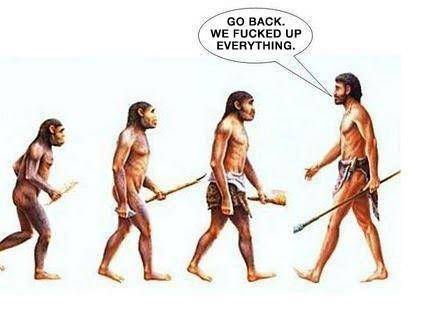
\includegraphics[height=0.8\paperheight]{devolution}}
    \only<3>{
\includegraphics[height=0.8\paperheight]{your-cat-is-evolving}}
}


\slide{C++ is becoming more and more complicated...}{
    \centering
    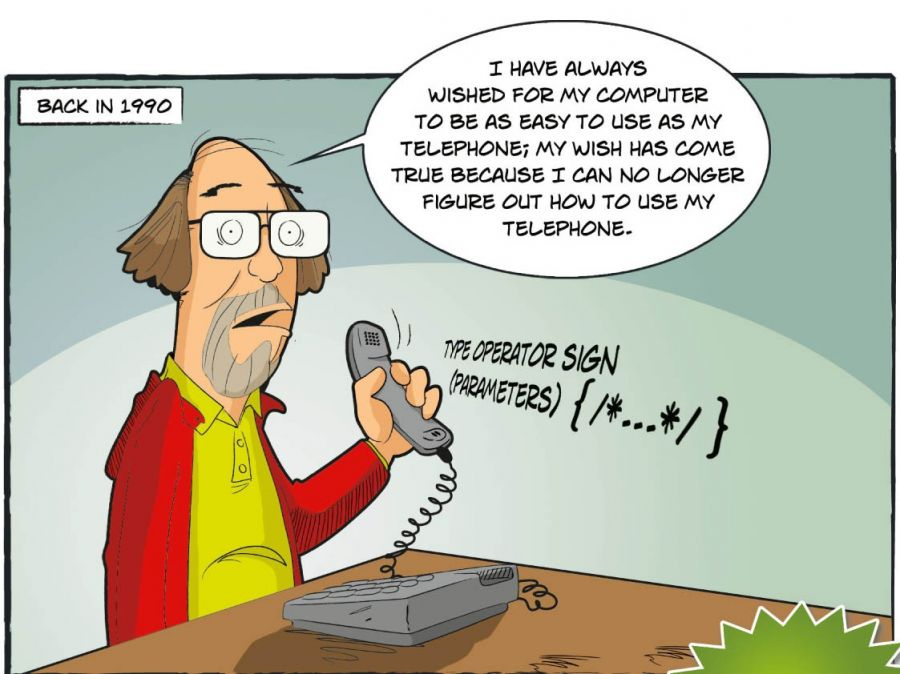
\includegraphics[height=0.8\paperheight]{bjarne-telephone}
}


%TODO: jakiś obrazek plątaniny porównujący skomplikowanie języka kiedyś i dziś
%TODO: jakieś zdjęcie z zarzutami
\slide{stdlib is poor}{
    \begin{columns}
        \begin{column}{0.3\textwidth}
            \begin{itemize}[<+->]
                \item Some people say that C++ standard library is small...
                \item In comparison to other languages
                \item Examples from presentation \textit{"One C++"} by Herb Sutter
                \item But it will grow in next standards
            \end{itemize}
        \end{column}
        \begin{column}{0.7\textwidth}
            \only<1>{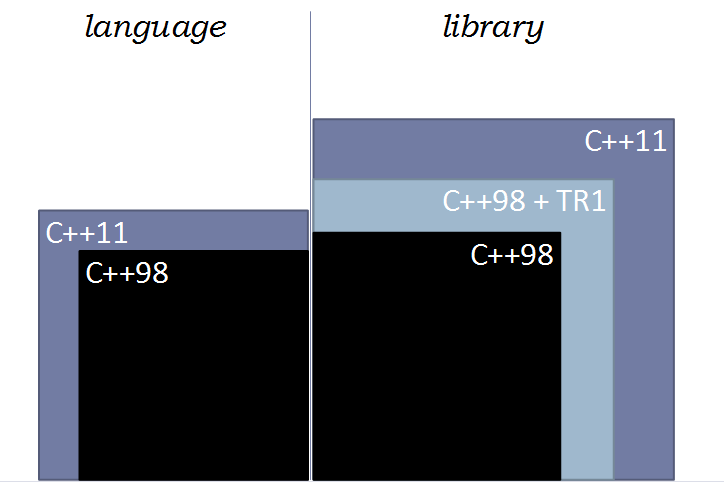
\includegraphics[height=0.7\paperheight]{cpp_libs}}
            \only<2>{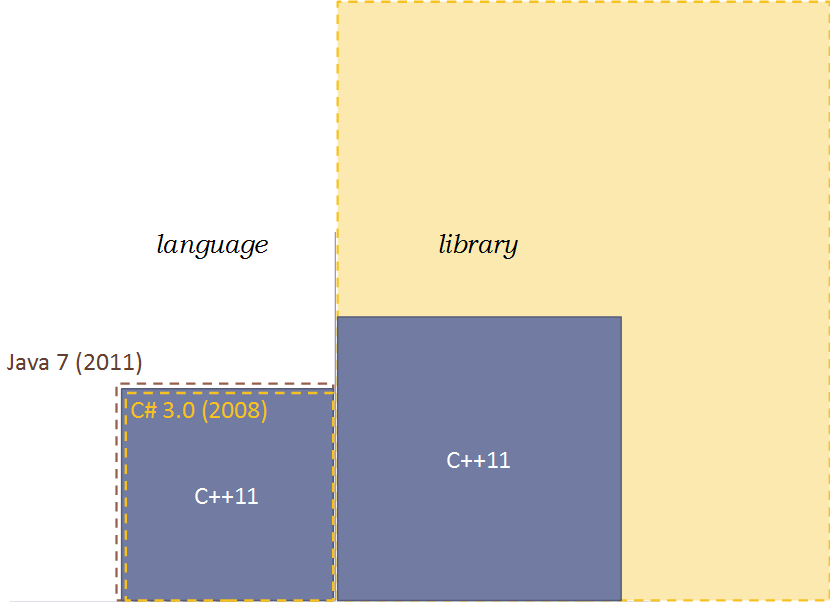
\includegraphics[height=0.85\paperheight]{cpp11_lib}}
            \only<3>{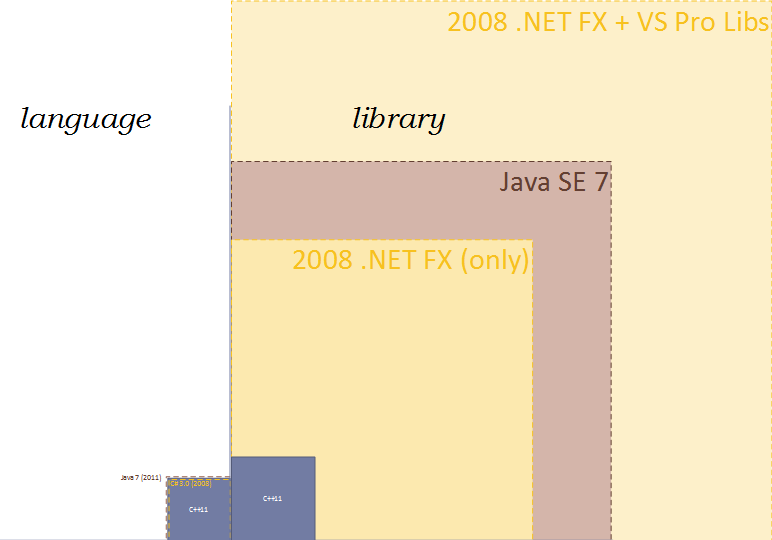
\includegraphics[height=0.8\paperheight]{cpp11_lib2}}\\
            \only<4>{\centering 
\includegraphics[height=0.8\paperheight]{bloated-jabbascript-frameworks}}
        \end{column}
    \end{columns}
}


\slide{C++ standard implementation delays}{
    \begin{table}
        %\caption{C++ users}
        \begin{tabular}{|l|r|r|} %TODO: Wiersz po wierszu niech się pojawia albo zaznaczenie zielonym
            \hline \textbf{Version} & \textbf{Standard} & \textbf{First implementation} \\
            \hline 
            \hline C84 & "the ARM" - 1989 & - \\
            \hline
            \hline C++98 & IX 1998 & 2003 (EDG + Dinkumware) \\
            \hline C++03 & X 2003 & ? \\
            \hline C++11 & IX 2011 & IV 2013 (clang3.3) \\
            \hline C++14 & III 2014 & XI 2013 (clang 3.4) \\
            \hline C++17 & ? & ? \\
            \hline
        \end{tabular}
    \end{table}
}


\slide{Free lunch is over}{
    \begin{columns}
    \begin{column}{0.57\textwidth}
        \begin{itemize}[<+->]
            \item Moore's law is no applicable anymore % Free lunch is over
            \item Processor speed doesn't rise
            \item We must go into concurrency
            \item We must write multithreaded apps
            \item We must write efficient and effective code
            \item Modern C++ facilitate above needs % Effective modern C++
            \item VM languages will not be faster than C++
            \item More and more mobile apps are written in C++
            \item Can C perform better? %TODO: QR kod do prezentacji Bartosza
        \end{itemize}
    \end{column}
    \begin{column}{0.43\textwidth}
        \only<1-5>{\centering 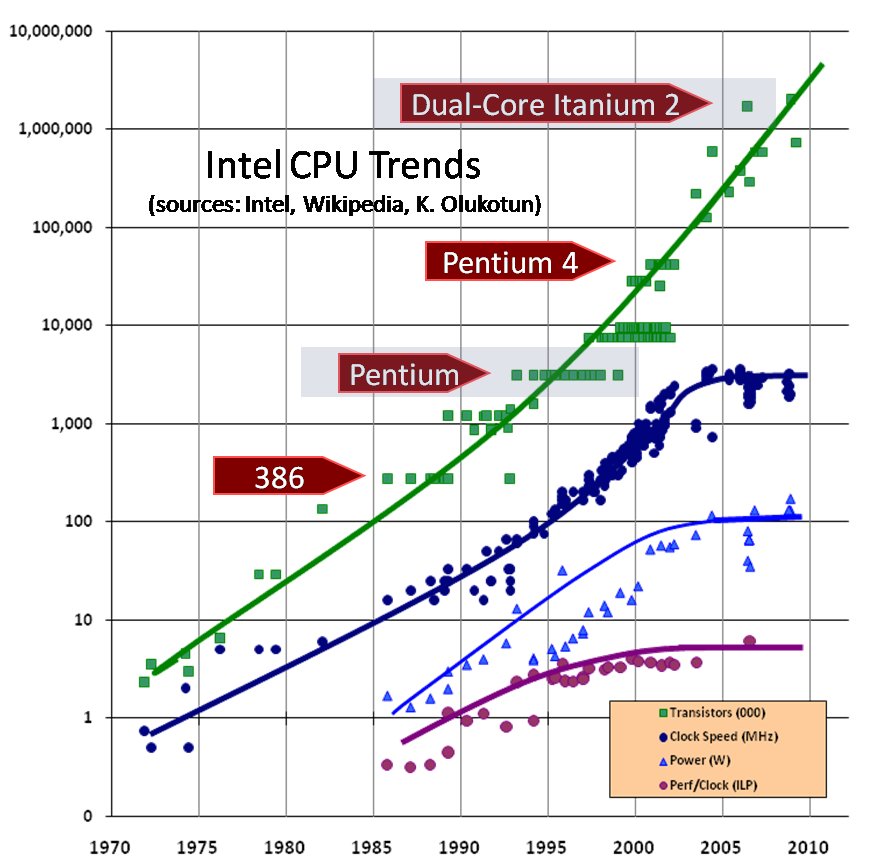
\includegraphics[height=0.6\paperheight]{free-lunch-is-over} \\
                   \scriptsize \url{http://www.gotw.ca/publications/concurrency-ddj.htm}}
        \only<6-8>{\centering 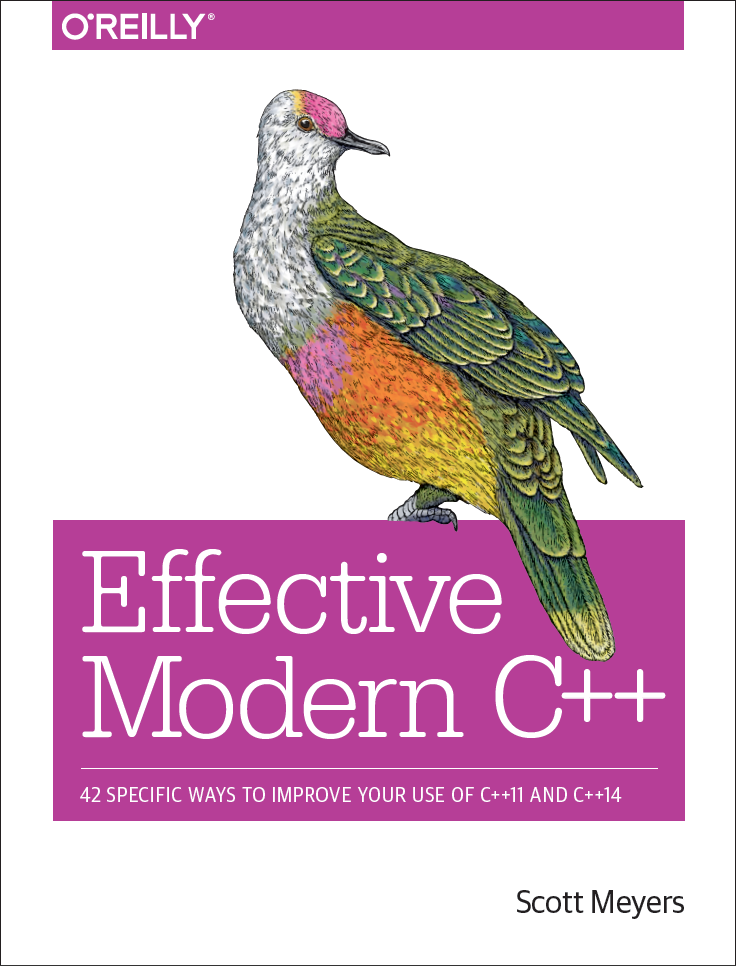
\includegraphics[height=0.7\paperheight]{effective-modern-cpp} \\
                   \scriptsize (This book cover is real)}
        \only<9>{\centering 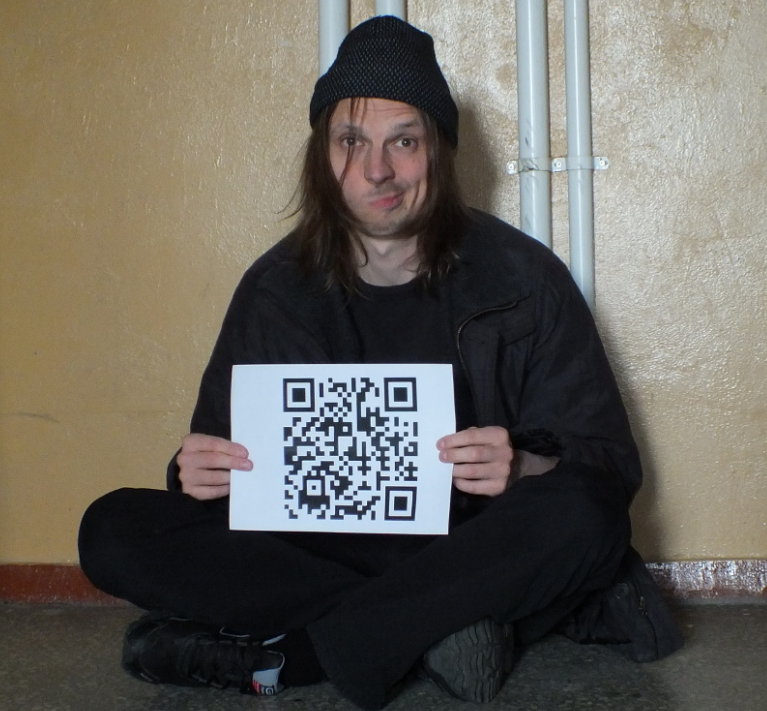
\includegraphics[height=0.6\paperheight]{szurgot} \\
                {\scriptsize Bartosz 'BaSz' Szurgot \\ C++ vs. C: The embedded perspective \\ code::dive 2015 }}
    \end{column}        
    \end{columns}
}